\documentclass{article}

\usepackage[affil-it]{authblk}
\usepackage{graphicx}
\usepackage{float}

\graphicspath{{../resources/}}

\title{Evolving a Sorting Algorithm with SNGP}
\author{Robin Lockyer}
\date{April 2019}
\affil{University of Liverpool}

\begin{document}
	
	\maketitle	
	
	\begin{abstract}
		
		Genetic programming is a technique for creating programmes not by writing them by hand, but instead by creating a population of random programmes and modifying them using an evolutionary algorithm. The desired result is that after several generations a programme that performs well at a given task is generated. GP has previously been used to successfully evolve sorting algorithms.
		
		Single node genetic programming is a variation on GP invented by Dr Jackson which structures the population of programmes in a manner that allows the use of dynamic programming when computing the result of the programmes in an effort to more efficiently generate a working solution. 
		
		This project aims to compare the effectiveness of the two methods in evolving a sorting algorithm.
		
	\end{abstract}

	\tableofcontents
	
	\section{Introduction}
	
		This project is was done for my project supervisor Dr David Jackson. The aim of this project is to attempt to evolve a sorting algorithm using node genetic programming (SNGP) and, if successful, compare the effectiveness of evolving sorting algorithms using standard genetic programming (GP) to evolving sorts with SNGP.
		
		The purpose of GP is to automate the creation of algorithms and programmes. This is done by applying a genetic algorithm to a population of random programmes so that successive generations of programmes improve at the desired characteristics until a functional programme is created.
		The standard approach to GP requires evaluating hundreds of programmes per generation over potentially thousands of generations and as such GP can take up a large amount of processing time. Several variations of GP have been created that try to reduce the amount of processing, including Linear Genetic Programming and Parallel Distributed GP \cite{poli_field_2008}.
		
		SNGP is one such variation devised by Dr Jackson in \textit{A New, Node-Focused Model for Genetic Programming} \cite{jackson_new_2012}. This variation makes use of a form of dynamic programming to re-use results of previously evaluated programmes. It has been shown that SNGP tends to perform better than standard GP in terms of processing time, solution rate, and solution size \cite{jackson_new_2012}. SNGP has reduced efficiency when dealing with problems with side-effects because this prevents re-use of evaluations, although it still performs better than GP at some problems with side effects \cite{jackson_single_2012}. 
		
		A sorting algorithm reads and manipulates an array of integers as it executes, and so must make use of side effects. Regular genetic programming has been shown to be capable of evolving a working sorting algorithm \cite{kinnear_evolving_1993,kinnear_generality_1993}. This makes evolving a sort a good problem to evaluate SNGP on as comparisons can be made with previous research.
	
	\section{Background}
	
		\subsection{Standard Genetic Programming}
		
			In standard GP, programmes are encoded as a tree of primitive functions and terminals.
			
			\begin{figure}[H]
				\centering
				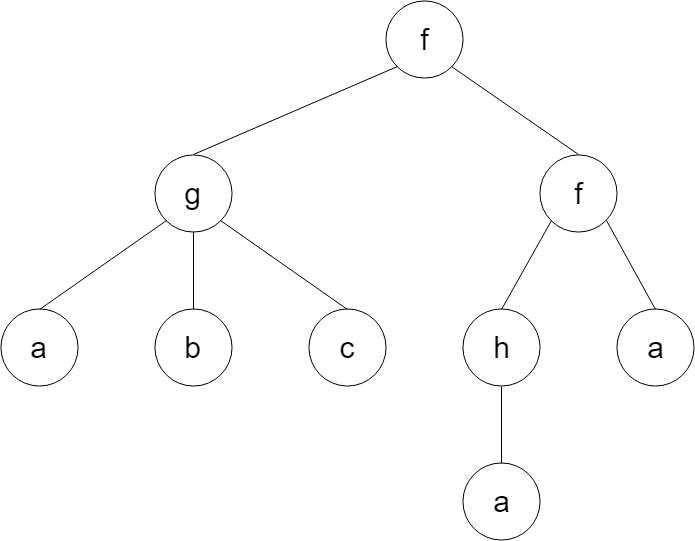
\includegraphics[width=0.5\textwidth]{1_gp_example_tree}
				\caption{This tree encodes the programme f( g( a, b, c ), f( h( a ), a ) ), where f, g, and h are functions and a, b, and c are terminals.}
			\end{figure}
			
			An initial population of random programmes is created
			
			\begin{figure}[H]
				\centering
				
\includegraphics[width=0.5\textwidth]{2_gp_example_population}
				\caption{An example GP population}
			\end{figure}
		
			Each member of the population is executed, evaluated, and given a fitness score
			
			\begin{figure}[H]
				\centering
				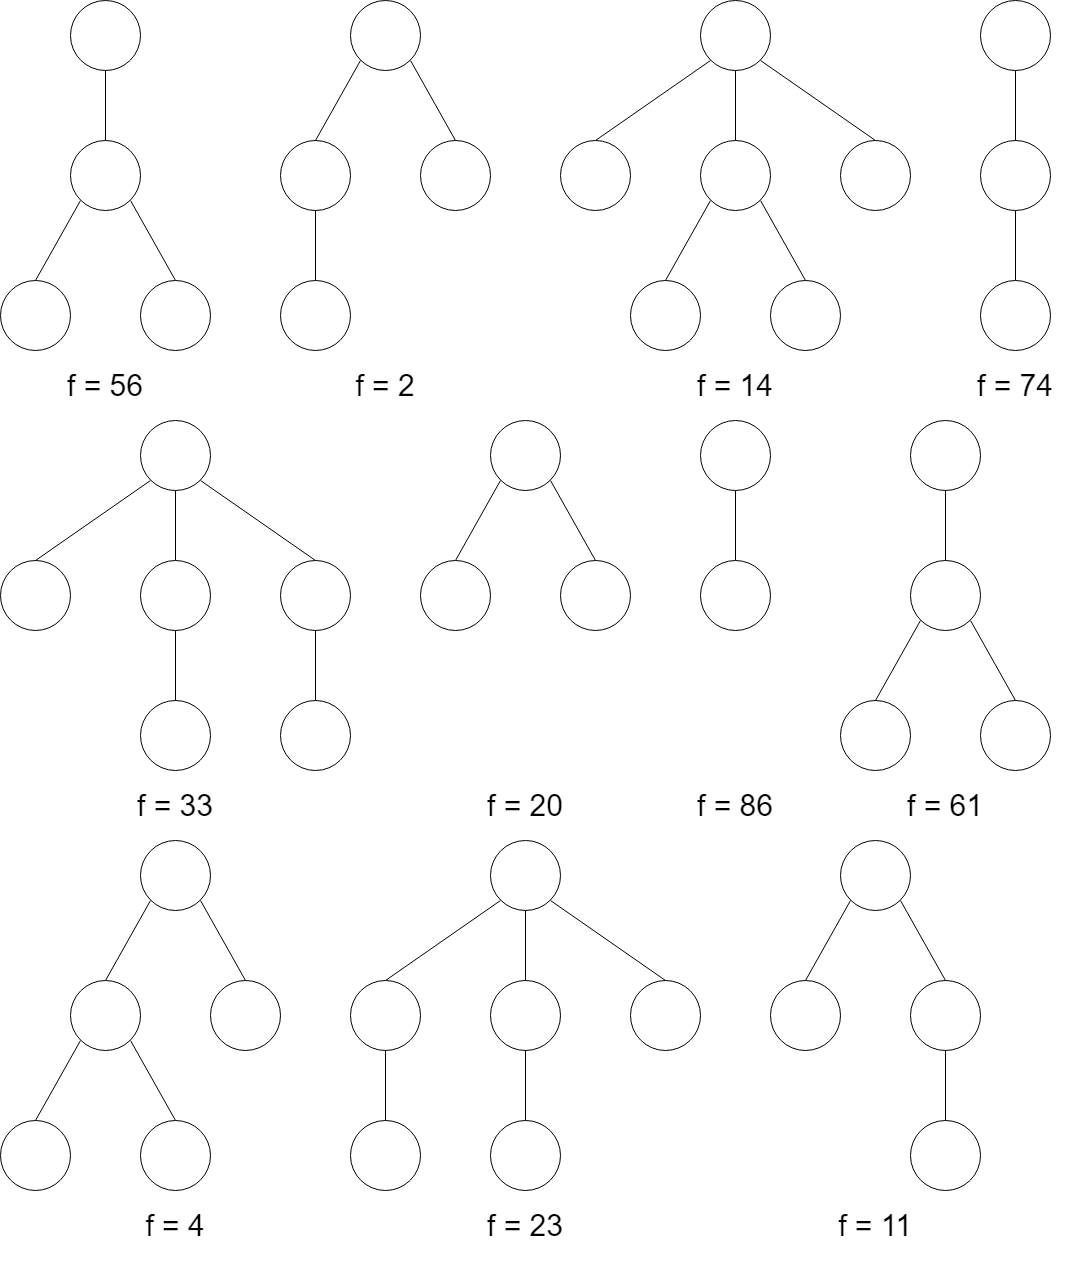
\includegraphics[width=0.5\textwidth]{3_gp_example_fitness}
				\caption{An example GP population with fitness scores}
			\end{figure}
		
			A new population is created by selecting some of the most fit members of the initial population and performing genetic operations on them to create new programmes.
			
			\begin{figure}[H]
				\centering
				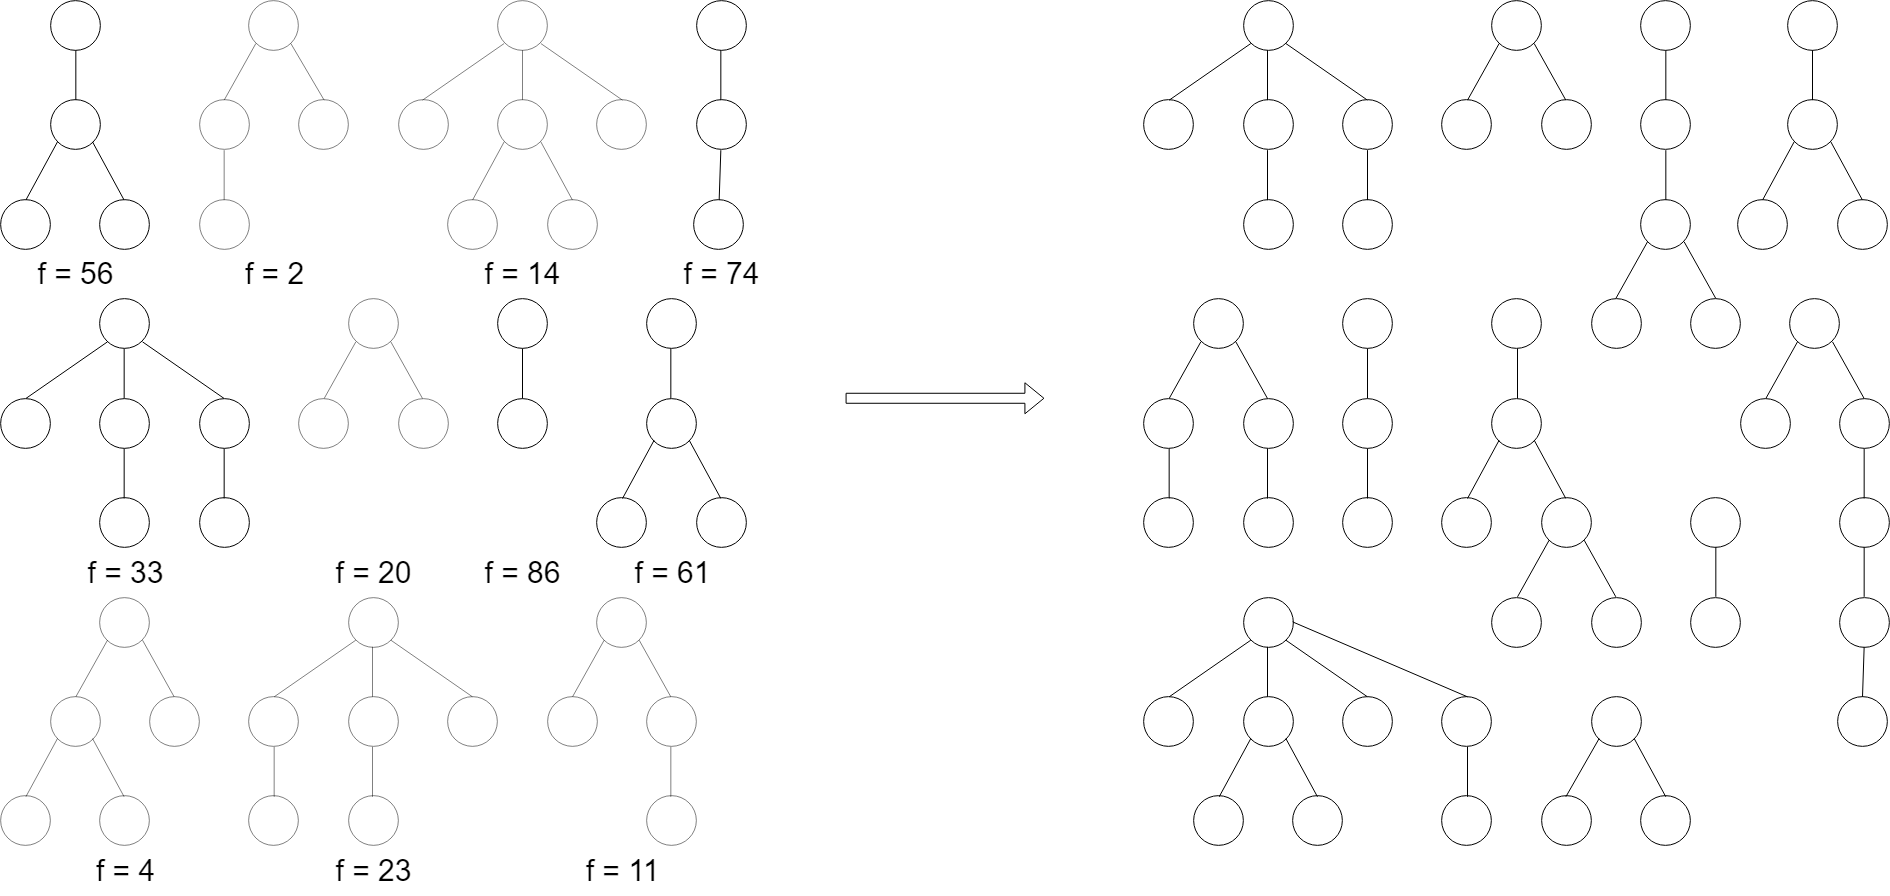
\includegraphics[width=0.5\textwidth]{4_gp_example_selection}
				\caption{An example GP population with fitness scores}
			\end{figure}
			
		\subsection{Single Node Genetic Programming}
		 
		
	
	\section{Data Required}
	
	\section{Design}
	
		\subsection{GP Implementation}
		
		\subsection{SNGP Implementation}
	
	\section{Realisation}
	
	\section{Results}
	
	\section{Evaluation}
	
	\section{Learning Points}
	
	\section{Professional Issues}
	
	\section{Bibliography}
	
		\bibliographystyle{acm}
		\bibliography{library}
	
	\section{Appendices}
		
\end{document}